\section{Száraz súrlódással csillapított rezgőrendszerek}

\subsection*{Mozgástörvény ábrázolása}
A száraz (Coulomb-) súrlódással rendelkező rendszer kitéréséből ($x_0>0$) történő indítás tipikus burkológörbéje egy lineárisan szűkülő cső, a mozgás pedig egy eltolt koszinuszos rezgésekből álló sorozat:
\begin{figure}[H]
    \centering
    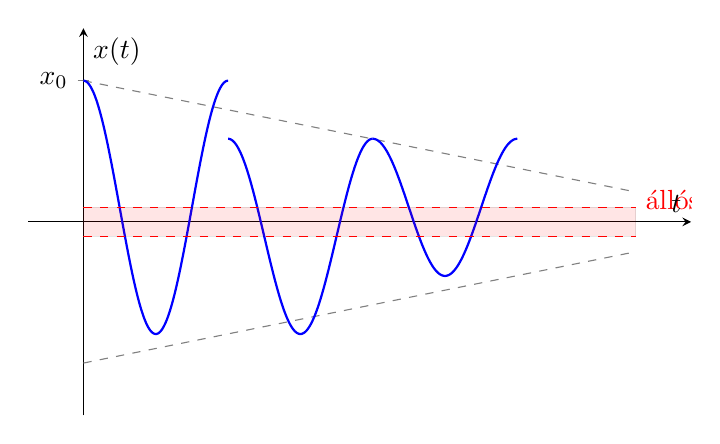
\begin{tikzpicture}
        \begin{axis}[
            width=10cm, height=6.5cm,
            axis lines=middle,
            xlabel={$t$},
            ylabel={$x(t)$},
            xmin=0, xmax=12,
            ymin=-4, ymax=4,
            xtick=\empty, ytick={3.5},
            yticklabels={$x_0$},
            enlargelimits=0.1,
            samples=200,
            domain=0:9.42
        ]
            % Linear envelopes
            \addplot[dashed, gray, domain=0:12] {3.5 - 0.23*x};
            \addplot[dashed, gray, domain=0:12] {-3.5 + 0.23*x};
            
            % Drawing piecewise dry friction exact motion
            % Period is pi. F/k offset changes every pi seconds. Amplitude drops by 2*F/k per half cycle (4*F/k per full cycle)
            \addplot[thick, blue, domain=0:3.1415] { (3.5 - 0.36)*cos(deg(2*x)) + 0.36 };
            \addplot[thick, blue, domain=3.1415:6.283] { (3.5 - 3*0.36)*cos(deg(2*x)) - 0.36 };
            \addplot[thick, blue, domain=6.283:9.424] { (3.5 - 5*0.36)*cos(deg(2*x)) + 0.36 };
            
            % Stop band
            \draw[fill=red, opacity=0.1] (0, -0.36) rectangle (12, 0.36);
            \draw[dashed, red] (0, 0.36) -- (12, 0.36);
            \draw[dashed, red] (0, -0.36) -- (12, -0.36);
            \node[red, right] at (12, 0.5) {állósáv $\left(\pm\frac{F_s}{k}\right)$};
        \end{axis}
    \end{tikzpicture}
    \caption{Száraz súrlódásos csillapítású mozgástörvény. A piros tartomány jelöli az állósávot.}
\end{figure}

\subsection*{Rezgések amplitúdócsökkenése és a beállás}
Ellentétben a viszkózus csillapítással, ahol exponenciálisan csökkent az amplitúdó, száraz súrlódás esetén a rezgések amplitúdói \textbf{lineáris összefüggés (aritmetikai sorozat)} szerint épülnek le. Minden egyes elmozdulási félperiódus alatt az amplitúdó pontosan $2\frac{F_s}{k}$-val csökken, ahol $F_s = \mu F_N$ a Coulomb-súrlódóerő, és $k$ a rugómerevség.

A beállás (megállás) akkor következik be, amikor a sebesség nullává válik valamelyik szélső (forduló) pontban, és az adott helyen a rugóban ébredő visszatérítő erő kisebb lesz, mint a maximális statikus tapadási súrlódóerő ($|k x| \le F_s$). Vagyis a mozgás nem tart végtelen ideig felületesen elvékonyodva (mint a viszkózus esetben), hanem \textbf{véges megfogható idő alatt} véget ér. A tömeg egy ún. \textbf{álló-sávon} (halott zónán, $x_{stop} \in [-\frac{F_s}{k}, \frac{F_s}{k}]$) belül bárhol végleg megállhat, aszimmetrikusan, nem feltétlenül az origóhoz rendelt abszolút egyensúlyi helyzetben.

\subsection*{A súrlódási tényező hatása}
\begin{itemize}
    \item \textbf{Beállásra gyakorolt hatás:} A súrlódási tényező ($\mu$) megadásával nő a tapadási és csúszási súrlódóerő nagysága. Ennek hatására a lineáris csökkenés (a burkológörbe meredeksége) sokkal agresszívabb lesz, emiatt a beállás (megállás) \textbf{jegyzetten hamarabb} áll be kevesebb lengés alatt. Továbbá megnő a piros "álló-sáv" vastagsága is, tehát annál pontatlanabb lesz a rendszer központosítása visszatéréskor.
    \item \textbf{Periódusidőre gyakorolt hatás:} Meglepő módon, a statikus Coulomb-féle száraz súrlódás \textbf{egyáltalán nem} befolyásolja a rezgés idejét a mozgás során! Habár a koszinusz görbe vízszintes tengelye eltolódik "szakaszonként", a lengés sajátkörfrekvenciája továbbra is a referencia (csillapítatlan) frekvencia marad: $\omega_d = \omega_n = \sqrt{\frac{k}{m}}$. Tehát a periódusidő $T = \frac{2\pi}{\omega_n}$ független a $\mu$ értékétől.
\end{itemize}
